\documentclass[a4paper,10pt]{article}
\usepackage{amsmath}
\usepackage{amssymb}
\usepackage{array}
\usepackage{graphicx}
\usepackage{url}
\usepackage[hidelinks]{hyperref}
\renewcommand{\UrlBreaks}{\do\/\do\_\do\.}

% The node's TeX installation has no geometry/booktabs/caption packages.
\setlength{\textwidth}{6.4in}
\setlength{\oddsidemargin}{-0.07in}
\setlength{\evensidemargin}{-0.07in}
\setlength{\topmargin}{-0.55in}
\setlength{\textheight}{9.6in}
\setlength{\parindent}{0pt}
\setlength{\parskip}{0.5em}
\renewcommand{\arraystretch}{1.12}
\graphicspath{{figures/}}

\newcommand{\garnet}{\texttt{GARNET}}
\newcommand{\code}[1]{\texttt{#1}}
\newcommand{\tablefile}[1]{\begin{center}\resizebox{\ifdim\width>\textwidth\textwidth\else\width\fi}{!}{\input{tables/#1}}\end{center}}
\newcommand{\Dt}{\tilde D}
\newcommand{\boxOrder}{2.00}
\newcommand{\spOrder}{2.00}
\newcommand{\cylOrder}{2.00}
\newcommand{\prismOrder}{2.00}
\newcommand{\skewOrder}{1.94}
\newcommand{\skewUncorrected}{-6227}
\newcommand{\reflMax}{1\times10^{-5}}
\newcommand{\Pref}{1.8485070086}
\newcommand{\kinfval}{1.2689196}
\newcommand{\biblisRef}{1.025258}
\newcommand{\biblisRefUnc}{0.5}
\newcommand{\biblisFine}{+3.0}
\newcommand{\biblisTwo}{1.02867}
\newcommand{\iaeaFine}{-17.8}
\newcommand{\vverFine}{-13.9}
\newcommand{\twiglFine}{-0.9}
\newcommand{\hpmrWorth}{5,581}
\newcommand{\hpmrWorthMid}{5,509}
\newcommand{\hpmrWorthCoarse}{5,246}
\newcommand{\hpmrWorthFine}{5,748}
\newcommand{\noabsSpread}{1.3}
\newcommand{\rThirtyTwoTime}{82}
\newcommand{\hpmrKout}{1.15034}
\newcommand{\hpmrKin}{1.08095}
\newcommand{\hpmrCellsSix}{11,880}
\newcommand{\runHost}{cn036}
\newcommand{\runDate}{2026-11-26}
\newcommand{\runNumpy}{2.3.5}
\newcommand{\runPython}{3.12.12}


\title{\textbf{\garnet{} Finite-Volume Diffusion and SP$_N$}\\
\large Theory, implementation, verification and validation}
\author{\garnet{} technical report}
\date{26 November 2026}

\begin{document}
\sloppy
\maketitle

\section*{Summary}

\garnet{} solves the multigroup neutron diffusion equation and its simplified
transport extensions (SP$_N$, SDP$_N$) with a cell-centred finite-volume method,
on CPUs through NumPy and on NVIDIA GPUs through CuPy, from one source. This
report states the equations, the discretization on every supported lattice, the
boundary conditions, and the eigenvalue and time-dependent algorithms as they
are implemented, and verifies and validates them with numbers recomputed for
this report.

\begin{itemize}
\item \textbf{Second order everywhere a closed form exists.} Bare boxes (diffusion
  and SP$_3$), a bare r--z cylinder and an extruded triangular-prism slab converge
  to their analytic eigenvalues with observed orders \boxOrder, \spOrder,
  \cylOrder{} and \prismOrder. Skewed unstructured triangles converge at order
  \skewOrder{} with the non-orthogonal correction; the plain two-point flux
  stalls at \skewUncorrected~pcm.
\item \textbf{Time integration has its nominal order.} Backward Euler, Crank--Nicolson,
  BDF2 and graded-start BDF3/BDF4 reach orders 1--4 on a six-family kinetics ramp
  with an independent reference.
\item \textbf{Benchmarks converge to their references.} On the finest meshes run
  here BIBLIS-2D is \biblisFine~pcm, IAEA-3D \iaeaFine~pcm and VVER-440
  \vverFine~pcm from FEMFFUSION solutions; TWIGL is \twiglFine~pcm from the
  published eigenvalue and matches the published transient powers to their three
  digits.
\item \textbf{HP-MR: explicit absorbers need equivalence, not refinement.} The 2-D
  heat-pipe microreactor model with 11-group ENDF/B-VIII.0 constants is
  mesh-converged within \noabsSpread~pcm without its control-drum absorbers. With
  them, the drum worth still moves by about 170~pcm between 0.97 and 0.48~cm
  triangles, because the B$_4$C thermal diffusion lengths are 0.002--0.05~cm. Drum
  worth comes from the S$_N$ references and SPH-DF equivalence, which the SPH audit
  shows to reproduce S$_N$ statics within 35~pcm and S$_N$ drum transients within
  0.25\,\% in final power.
\end{itemize}

Transport (S$_N$), SPH equivalence, thermal coupling and the GPU performance
studies have their own reports, listed in Section~\ref{sec:further}.

\tableofcontents

% ---------------------------------------------------------------------------
\section{Equations}
\label{sec:equations}

\subsection{Multigroup diffusion}

With $G$ energy groups, the scalar flux $\phi_g(\mathbf r)$ of group $g$ obeys
\begin{equation}
-\nabla\cdot D_g\nabla\phi_g + \Sigma_{r,g}\,\phi_g
  = \sum_{g'\neq g}\Sigma_{s,g'\to g}\,\phi_{g'}
  + \frac{\chi_g}{k}\sum_{g'}\nu\Sigma_{f,g'}\,\phi_{g'},
\label{eq:diffusion}
\end{equation}
with $D_g$ the diffusion coefficient, $\Sigma_{r,g} = \Sigma_{a,g} +
\sum_{g'\neq g}\Sigma_{s,g\to g'}$ the removal cross section, $\Sigma_{s}$ the
scattering matrix, $\nu\Sigma_f$ the fission production and $\chi$ the fission
spectrum. In operator form $M\phi = k^{-1}F\phi$; the largest eigenvalue $k =
k_\mathrm{eff}$ and its positive eigenvector are sought.

\subsection{\texorpdfstring{SP$_3$, SP$_N$ and SDP$_N$}{SP3, SPN and SDPN}}

The SP$_3$ equations of Brantley and Larsen~\cite{brantley2000} are solved in
the unknowns $\Phi_1 = \phi_0 + 2\phi_2$ and $\phi_2$:
\begin{align}
-\nabla\cdot D_1\nabla\Phi_1 + \Sigma_0\Phi_1 - 2\Sigma_0\phi_2 &= q_0,\\
-\nabla\cdot D_2\nabla\phi_2 + \left(\Sigma_t + \tfrac45\Sigma_0\right)\phi_2
  - \tfrac25\Sigma_0\Phi_1 &= -\tfrac25 q_0,
\end{align}
with $D_1 = D$, $D_2 = 9/(35\Sigma_t)$ and $\Sigma_0$ the within-group removal
($1/(5\Sigma_t)$ replaces $D_2$ for SDP$_1$). $q_0$ carries the scattering and
fission sources of Eq.~(\ref{eq:diffusion}). Multiplying the second equation by
5 makes both coupling terms $-2\Sigma_0$, so the $2\times2$ block is symmetric
positive definite and is solved by one conjugate-gradient (CG) iteration per group.

The general SP$_N$ ($N = 1, 3, 5, 7$) and SDP$_N$ ($N = 1, 2, 3$) solvers use the
form of Carre\~no et al.~\cite{carreno2024}
\begin{equation}
-\nabla\cdot D_i\nabla U_i + \sum_j A_{ij}U_j = s_i,\qquad
A_{ij} = c^{(1)}_{ij}\Sigma_0 + \sum_{m\ge2}c^{(m)}_{ij}\Sigma_t,
\end{equation}
with $D_0 = D$, $D_i = 1/((4i+3)\Sigma_t)$ for $i\ge1$, and the scalar flux
$\phi_0 = \sum_j c^{(1)}_{0j}U_j$. The SP$_N$ coefficient tables are symmetric.
SDP$_1$ and SDP$_2$ are symmetrized by a diagonal similarity and SDP$_3$ by a
congruence that diagonalizes the coupling (Section~\ref{sec:inner}).

\subsection{Kinetics}

The time-dependent problem adds the neutron speed $v_g$ and $I$ delayed-neutron
precursor families $C_i$:
\begin{align}
\frac{1}{v_g}\frac{\partial\phi_g}{\partial t} &= \nabla\cdot D_g\nabla\phi_g
  - \Sigma_{r,g}\phi_g + \sum_{g'\ne g}\Sigma_{s,g'\to g}\phi_{g'}
  + \Bigl(\chi_g - \sum_i\beta_i\chi_{d,ig}\Bigr)S
  + \sum_i\chi_{d,ig}\lambda_iC_i,\\
\frac{\partial C_i}{\partial t} &= \beta_iS - \lambda_iC_i,\qquad
S = \frac{1}{k_0}\sum_g\nu\Sigma_{f,g}\phi_g .
\end{align}
Dividing the fission source by the initial eigenvalue $k_0$ makes the initial
state an exact equilibrium; the precursors start at $C_i = \beta_iS/\lambda_i$
and the power is normalized to one. Delayed spectra $\chi_{d}$ are optional,
shared or per family.

% ---------------------------------------------------------------------------
\section{Finite-volume discretization}
\label{sec:discretization}

\subsection{Cell balance and the two-point flux}

Integrating Eq.~(\ref{eq:diffusion}) over a cell $i$ of volume $V_i$ turns the
divergence into the sum of the face currents. Across a face of area $A$ between
cells $i$ and $j$, whose centroids lie at normal distances $\delta_i$ and
$\delta_j$ from the face, continuity of the flux and of the current gives the
two-point flux
\begin{equation}
J_{i\to j} = \frac{A}{\delta_i/D_i + \delta_j/D_j}\,(\phi_i - \phi_j).
\label{eq:tpfa}
\end{equation}
It is exact for piecewise-constant $D$ and a linear flux on each side. On the
structured lattices $\delta_i = \delta_j = d/2$ with $d$ the centroid spacing,
and Eq.~(\ref{eq:tpfa}) becomes $\Dt A(\phi_i-\phi_j)/d$ with the harmonic mean
$\Dt = 2D_iD_j/(D_i+D_j)$. A strong absorber ($D\to0$) closes the face, as it
should. Dividing by the cell volume gives one coupling coefficient per face,
$w = \Dt A/(dV)$, and the cell balance becomes a stencil:
\begin{equation}
(A\phi)_i = \Bigl(\Sigma_{r,i} + \sum_{f}w_f\Bigr)\phi_i - \sum_f w_f\,\phi_{\mathrm{nbr}(f)}.
\end{equation}

Table~\ref{tab:lattices} lists the geometry factors. The hexagonal and
triangular coefficients follow from the face length, the centroid spacing and
the cell area; they were checked against the code by direct derivation.

\begin{table}[htbp]
\begin{center}
\small
\begin{tabular}{llllll}
\hline
lattice & cell & face & $d$ & $w$ & Robin term per volume\\
\hline
Cartesian & box, spacing $\Delta$ & $\Delta^2$ & $\Delta$ & $\Dt/\Delta^2$ &
  $2D\alpha/(\Delta(\Delta\alpha + 2D))$\\
triangular & equilateral, side $h$ & $h$ & $h/\sqrt3$ & $4\Dt/h^2$ &
  $8D\alpha/(h(h\alpha + 2\sqrt3D))$\\
hexagonal & flat-to-flat pitch $p$ & $p/\sqrt3$ & $p$ & $2\Dt/(3p^2)$ &
  $4D\alpha/(3p(p\alpha + 2D))$\\
axial (prisms) & layer $\Delta z$ & cell base & $\Delta z$ & $\Dt/\Delta z^2$ &
  $2D\alpha/(\Delta z(\Delta z\alpha + 2D))$\\
\hline
\end{tabular}
\end{center}
\caption{Coupling coefficients and boundary terms on the structured lattices.
Triangular and hexagonal faces are lengths per unit height; both lattices are
extruded into prisms by the axial row.}
\label{tab:lattices}
\end{table}

\paragraph{Cylindrical r--z.} The equation is multiplied by the cell-centre radius
$r_c = (i+\frac12)\Delta r$, which is the annulus volume up to $2\pi\Delta r\Delta z$:
radial couplings carry the face radius $r_f = i\Delta r$, axial couplings and the
removal term carry $r_c$. The axis face has $r_f = 0$ and therefore no
boundary term. The weighted operator is symmetric; a non-symmetric divergence form
(\code{symmetric=False}) is kept for comparison.

\paragraph{Unstructured meshes.} \code{garnet.mesh} reads Gmsh~2.2 meshes of
triangles and quadrilaterals (2-D) or tetrahedra, hexahedra and prisms (3-D), and
accepts hanging nodes. The face coefficient is Eq.~(\ref{eq:tpfa}) with the
normal distances, volume-integrated. On non-orthogonal faces, where the line
between centroids is not normal to the face, the two-point flux alone is
inconsistent: its error does not vanish under refinement. \garnet{} adds the
tangential flux from least-squares cell gradients, interpolated to the face. The
eigenvalue solver lags this term into the source, which keeps the operator
symmetric; the transient mesh operator applies it implicitly, which makes the
operator non-symmetric and calls for GMRES. On orthogonal meshes the correction
is zero and is skipped.

\paragraph{Active masks.} A reactor that does not fill its array (a hexagonal core
on a triangular lattice, an octagonal core on a Cartesian grid) uses a boolean
active mask. Faces between an active and an inactive cell carry no coupling; the
active cell receives the boundary term of \code{mask\_bc} (vacuum by default),
and inactive cells are decoupled with a unit diagonal and stay at zero.

\subsection{Boundary conditions}
\label{sec:bc}

Every boundary obeys one Robin law, $J_\mathrm{net} = \alpha\,\phi_s$, the net
outward current proportional to the surface flux. Eliminating $\phi_s$ between it
and the half-cell flux $J = D(\phi_c - \phi_s)/\delta$ leaves a non-negative
diagonal term $(A/V)\,\alpha D/(\alpha\delta + D)$, the last column of
Table~\ref{tab:lattices}. The physics is selected by $\alpha$:

\begin{center}
\begin{tabular}{lll}
\hline
condition & $\alpha$ & meaning\\
\hline
reflective & 0 & no net current: symmetry plane\\
vacuum (Marshak) & $\frac12$ & no incoming neutrons\\
user value & $\alpha\ge0$ & e.g.\ an albedo $\beta$ gives $\alpha = (1-\beta)/(2(1+\beta))$\\
zero flux & $\infty$ & Dirichlet limit, term $2D/\Delta^2$ on a Cartesian face\\
\hline
\end{tabular}
\end{center}

\garnet{} takes $\alpha$ itself; the albedo relation is for the user's
convenience. SP$_N$ and SDP$_N$ moments are coupled at a vacuum face by the
Marshak conditions $J = G\,U$ with a full matrix $G$ (for SP$_3$, $J_1 =
\frac12\Phi_1 - \frac38\phi_2$, $J_2 = -\frac{3}{40}\Phi_1 + \frac{21}{40}\phi_2$).
This coupled condition is the default on Cartesian grids; elsewhere, and for the
dedicated SDP$_1$ solver, each moment gets its own $\alpha = \frac12$ term.

\subsection{Matrix-free application}
\label{sec:matrixfree}

On a structured lattice the neighbour of every cell in a given direction is the
same array shifted by one index. Applying the operator is therefore a few
element-wise operations on shifted views; the Cartesian kernel is
\begin{verbatim}
out = diag * phi
out[1:, :, :]  -= wx * phi[:-1, :, :]     # west neighbours of all cells
out[:-1, :, :] -= wx * phi[1:, :, :]      # east
...                                       # south, north, below, above
\end{verbatim}
The coupling arrays and the diagonal are built once per group with materials,
masks and boundary terms folded in, so the loop has no branches and no index
lists. The triangular lattice couples its two sublattices (``up'' and ``down''
triangles) at three fixed offsets, the hexagonal lattice uses six
axial-coordinate offsets, and extrusion adds the two axial terms. On a GPU the
Cartesian and triangular stencils run as one fused CuPy element-wise kernel each.
Unstructured meshes use a padded neighbour table (ELLPACK) and a gather.

Every structured diffusion operator is symmetric, because a face coupling is
shared by its two cells, and diagonally dominant, strictly so in any row with
removal or a leaking boundary. It is therefore symmetric positive definite, which
licenses CG. Discontinuity factors, the implicit non-orthogonal correction, the
r--z divergence form and SDP$_N$ with coupled Marshak boundaries make the
operator non-symmetric.

% ---------------------------------------------------------------------------
\section{Eigenvalue solution}
\label{sec:eigen}

\subsection{Outer iteration}

The eigenvalue problem is solved by power iteration on the fission source. Each
outer iteration sweeps the groups in order $g = 1,\dots,G$ (Gauss--Seidel): group
$g$ uses the updated fluxes of the faster groups and the previous fluxes of the
slower ones, so up-scattering is lagged by one outer. The eigenvalue is updated by
$k \leftarrow k\,S_\mathrm{new}/S$ with $S$ the total fission source, and the
source error is $\|f_\mathrm{new}/S_\mathrm{new} - f/S\|_2/\|f_\mathrm{new}/S_\mathrm{new}\|_2$.

\paragraph{Stopping test.} Power iteration converges at the dominance ratio
$\rho$, so a small change between iterates can hide a large error. \garnet{}
estimates $\hat\rho$ from the last four source errors and tightens each
tolerance to $\varepsilon(1-\hat\rho)$, which bounds the remaining error rather
than the last step. It also requires the inner tolerance to have reached the
outer one. Defaults are $10^{-7}$ on $k$ and $10^{-6}$ on the source
(the \code{Model} API defaults to $10^{-6}$ and $10^{-5}$).

\paragraph{Anderson acceleration.} The fission-source fixed point is accelerated
by Anderson mixing of depth 8~\cite{walker2011}, with Tikhonov regularization and
safeguards: the history restarts when the error grows by more than 10\,\%, and
plain power iteration takes over after three restarts that fail to halve it.
The adjoint solve does not use it.

\paragraph{Wielandt shift.} For loosely coupled cores the optional Wielandt shift
solves $(M - \lambda_sF)\Psi = (\lambda - \lambda_s)F\Psi$ with $\lambda_s = 1/k_s$
slightly above the fundamental eigenvalue, which reduces the dominance ratio. The
shifted multigroup system is solved by flexible GMRES, right-preconditioned by a
Gauss--Seidel group sweep. A fixed shift $k_s = k + \delta k$ is the default;
an adaptive mode tunes $\delta k$ to a target number of inner iterations.

\subsection{Inner solves}
\label{sec:inner}

Each group solve is warm-started from the previous outer and solved to a relative
tolerance that follows the outer error,
$\max\bigl(\min(10^{-3}, 0.1\,e_\mathrm{src}), 10^{-10}\bigr)$, so early outers
are cheap. Symmetric operators use preconditioned CG. Jacobi (inverse diagonal)
preconditioning is the default; a damped Neumann polynomial
$\sum_{k<d}(I-\omega D^{-1}A)^k\,\omega D^{-1}$, with $\omega = 2/(\lambda_\mathrm{min}
+ \lambda_\mathrm{max})$ estimated by twelve Lanczos steps, is available.
Non-symmetric operators use GMRES or BiCGStab.

The SP$_3$ block is solved by block CG after the scaling above. SDP$_3$ has no
diagonal symmetrization; a congruence $R = H^{1/2}$, $S = Q^{-1}H^{-1/2}$, with
$H$ symmetric positive definite and $HT_k = T_k^\top H$ for the coupling
matrices, decouples it into scalar diffusion problems on reflective or zero-flux
boundaries. With coupled Marshak boundaries the SDP$_N$ blocks are
non-symmetric and use GMRES; SP$_N$ blocks stay symmetric and use CG.

\subsection{Adjoint}

The adjoint solve exchanges $\chi$ and $\nu\Sigma_f$, transposes the
scattering matrix and applies the transpose of any non-symmetric operator.
First-order perturbation theory evaluates the perturbed operators $M'$, $F'$ on
the unperturbed forward and adjoint fluxes, $\Delta\rho = 1/k -
\langle\phi^*, M'\phi\rangle/\langle\phi^*, F'\phi\rangle$; it is available for the
scalar-flux solvers.

% ---------------------------------------------------------------------------
\section{Time-dependent solution}
\label{sec:transient}

\subsection{Time schemes and precursors}

All schemes share one step equation,
\begin{equation}
\bigl(A + a_0\theta\bigr)u^{n+1} = S^{n+1} + a_0\theta\,\Psi^n,\qquad
\theta = \frac{1}{v\,\Delta t},
\end{equation}
so the spatial solver sees only a diagonal shift $a_0\theta$ and a carried field
$\Psi$. Backward Euler has $a_0 = 1$, $\Psi = u^n$; BDF$q$ ($q\le6$) has its
leading coefficient $a_0$ and history $\Psi = H/a_0$, with variable-step
coefficients from the step history; the $\theta$-method (Crank--Nicolson at
$\theta = \frac12$) carries $\Psi^{n+1} = u + ((1-w)/w)(u-\Psi^n)$. The precursor
equations are discretized with the same formula and eliminated:
$C_i^{n+1} = (\Delta t\,\beta_iS^{n+1} + H_i)/(a_0 + \lambda_i\Delta t)$. The
resulting fission weight $\beta_ia_0/(a_0+\lambda_i\Delta t)$ and delayed source
enter the step equation; no separate precursor solve is needed, and the initial
equilibrium is preserved exactly by any BDF order.

A multistep formula has no history on its first steps. Fixed-step BDF3--BDF6 ramp
their order from one and are then only second order overall;
\code{bdf\_startup="graded"} grows the first steps geometrically and restores
orders three and four. Adaptive BDF estimates the local error from a polynomial
predictor, chooses the next step by the rule of Cherezov et
al.~\cite{cherezov2025}, rejects and halves failed steps, and can select the order
automatically. Backward Euler is the default scheme; SP$_N$ transients use
backward Euler only.

\subsection{The step solve}

Each step is a fixed-source multigroup problem whose operator is the steady one
plus the positive shift, still symmetric positive definite and better conditioned.
The default fixed-point solver sweeps the groups with warm-started PCG and
accelerates the within-step fission source by Anderson mixing (depth~5); a
monolithic alternative solves the whole multigroup block with flexible GMRES,
preconditioned by group sweeps. Quasi-static methods (adiabatic and
predictor--corrector IQS) factor the flux into an amplitude and a slowly varying
shape and are described with the transient API.

% ---------------------------------------------------------------------------
\section{CPU and GPU execution}

The solvers are written against the NumPy array interface, which CuPy mirrors:
\code{device="cpu"} or \code{"gpu"} selects the array module, and the physics code
is identical on both. A stencil application reads a few arrays and writes one
with about two floating-point operations per value read, so large solves are
limited by memory bandwidth; small grids are limited by kernel-launch latency.
Both favour the matrix-free form: it reads only coefficients and fluxes, in
contiguous order, and the fused kernels of Section~\ref{sec:matrixfree} remove
the intermediate arrays (6--7$\times$ faster stencil, 1.3--2.4$\times$ faster solves
on a T4). The PCG state and scalars stay on the device; the host reads one
convergence check every \code{check\_every} iterations. CUDA-graph capture of the
PCG loop and single-precision preconditioning are available as options.
Single-device execution is the current scope.

The verification and validation numbers below were computed with one thread on
two reserved cores of shared merlin7 CPU nodes (\code{daily} partition; the host
of each study is recorded in \code{data/environment*.json}), Python \runPython,
NumPy \runNumpy, \runDate. Times are the fastest of three identical runs, except the
transients and the HP-MR sweep, which ran once. GPU timings are in the
FEMFFUSION comparison~\cite{garnetfemffusion}.

% ---------------------------------------------------------------------------
\section{Verification}
\label{sec:verification}

Verification checks that the equations are solved correctly, against exact
solutions of the same equations. All solves here use tolerances $10^{-10}$ on $k$
and $10^{-9}$ on the source, far below the errors reported.

\subsection{Eigenvalue convergence}

Table~\ref{tab:verification} and Figure~\ref{fig:convergence} compare \garnet{}
with closed-form eigenvalues:
\begin{itemize}
\item a bare $90\times90\times90$~cm cube with two-group data and zero-flux faces, for
  diffusion and SP$_3$ (\code{k\_bare\_box}, \code{k\_bare\_box\_sp3});
\item a bare one-group cylinder ($R = 80$~cm, $H = 160$~cm) on an r--z grid, against
  $k = \nu\Sigma_f/(\Sigma_a + D[(j_{0,1}/R)^2 + (\pi/H)^2])$;
\item a 120~cm slab built from triangular prisms with reflective sides and zero-flux
  ends, against the one-dimensional buckling eigenvalue;
\item a bare 10~cm square meshed by cutting every cell of an $n\times n$ grid along
  the same diagonal: every face is non-orthogonal.
\end{itemize}

\begin{table}[htbp]
\tablefile{verification}
\caption{Eigenvalue convergence against analytic references. Error $= 10^5(k -
k_\mathrm{exact})$; order $=\log_2$ of successive error ratios for halved
spacing. Outers, inners (operator applications) and time are the cost of one solve.}
\label{tab:verification}
\end{table}

\begin{figure}[htbp]
\begin{center}
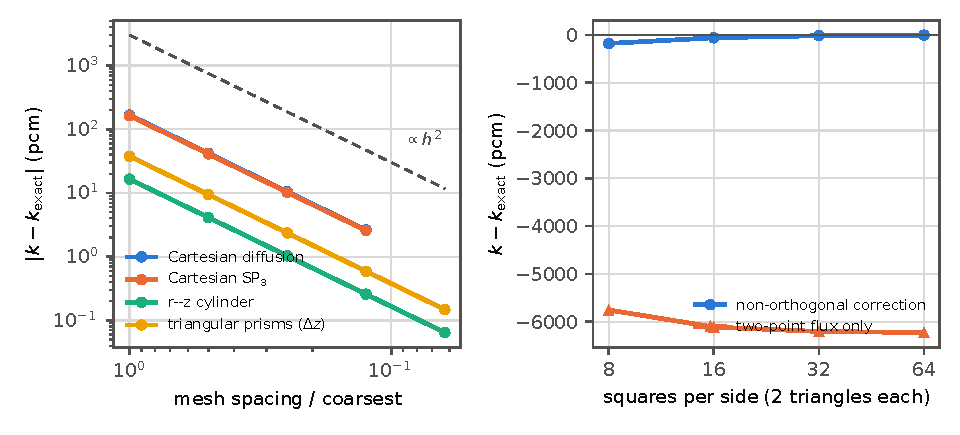
\includegraphics[width=\textwidth]{convergence.pdf}
\end{center}
\caption{Left: eigenvalue error against relative mesh spacing for the structured
lattices; the dashed line is second order. Right: signed error on skewed
triangles with and without the non-orthogonal correction.}
\label{fig:convergence}
\end{figure}

Every structured lattice converges at second order, the expected order of a
cell-centred two-point scheme. On the skewed triangles the plain two-point flux
does not converge: it settles near \skewUncorrected~pcm. The correction restores
second order.

With reflective boundaries there is no leakage and the flux is flat, so $k$ must
equal $k_\infty = \kinfval$ exactly; Table~\ref{tab:reflective} shows the
Cartesian, triangular-prism and hexagonal-prism operators within
$\reflMax$~pcm, the solver tolerance.

\begin{table}[htbp]
\tablefile{reflective}
\caption{Reflective boundaries on every lattice: $k = k_\infty$ to solver tolerance.}
\label{tab:reflective}
\end{table}

\subsection{Time integration}

A homogeneous medium with reflective boundaries has no spatial error, and its
kinetics reduce to ordinary differential equations. A one-group medium with six
delayed families and a reactivity ramp of 0.615\,\$ over 0.2~s is integrated by
\garnet{} and, independently, by a Radau solver at relative tolerance
$10^{-12}$, giving $P(0.2\,\mathrm{s}) = \Pref$. Table~\ref{tab:kinetics} and
Figure~\ref{fig:kinetics} give the end-of-ramp error. Each scheme reaches its
nominal order; Crank--Nicolson is second order on this smooth ramp, and BDF3 and
BDF4 need the graded start to do so.

\begin{table}[htbp]
\tablefile{kinetics}
\caption{Relative error of $P(0.2\,\mathrm{s})$ on the kinetics ramp; order from
the two finest steps.}
\label{tab:kinetics}
\end{table}

\begin{figure}[htbp]
\begin{center}
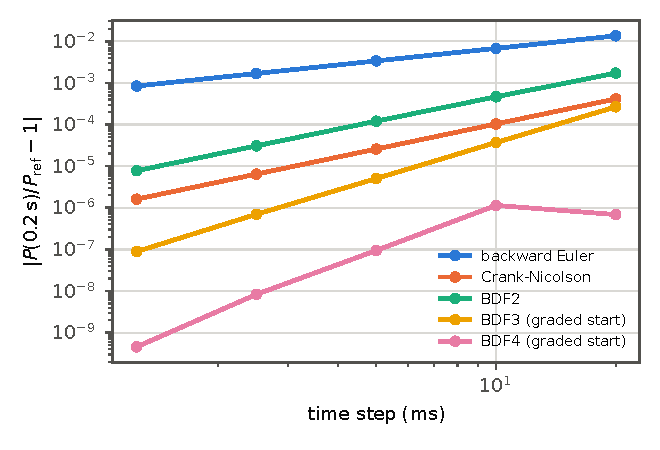
\includegraphics[width=0.62\textwidth]{kinetics.pdf}
\end{center}
\caption{End-of-ramp error against time step for each scheme.}
\label{fig:kinetics}
\end{figure}

The test suite carries many more checks: SP$_N$/SDP$_N$ derivations and operator
symmetry, adjoint transposes, boundary conditions, mesh readers, point-kinetics
equivalence and BDF history handling. They are mapped to their features in the
verification and validation record~\cite{vvrecord}.

% ---------------------------------------------------------------------------
\section{Validation}
\label{sec:validation}

Validation compares \garnet{} with reference solutions of published reactor
problems. Table~\ref{tab:validation} refines each problem towards its reference;
Figure~\ref{fig:validation} plots the errors.

\begin{itemize}
\item \textbf{BIBLIS-2D}: a two-group PWR core with vacuum boundary on a
  Cartesian grid. The reference, $k = \biblisRef \pm \biblisRefUnc$~pcm, is the
  Richardson limit of FEMFFUSION~\cite{femffusion} degree-3 finite elements at
  three refinements, computed for this report with FEMFFUSION's own BIBLIS input;
  a degree-4 solution agrees within 0.6~pcm. (A constant 1.0287 previously
  carried as the published value is \garnet's own result at two cells per
  assembly, \biblisTwo.)
\item \textbf{IAEA-3D}~\cite{finnemann1977}: a two-group PWR core with albedo
  boundaries. Reference: the FEMFFUSION degree-3 limit $1.0290729 \pm 0.1$~pcm
  of the FEMFFUSION comparison~\cite{garnetfemffusion}.
\item \textbf{VVER-440}: a 2-D hexagonal-assembly core on body-fitted triangles
  ($6r^2$ triangles per assembly). Reference: FEMFFUSION's diffusion solution.
\item \textbf{TWIGL}~\cite{hageman1969}: a two-group seed--blanket core, with the
  published static eigenvalue and transient powers.
\end{itemize}

\begin{table}[htbp]
\tablefile{validation}
\caption{Eigenvalue against the reference of each benchmark; $\Delta k = 10^5(k -
k_\mathrm{ref})$.}
\label{tab:validation}
\end{table}

\begin{figure}[htbp]
\begin{center}
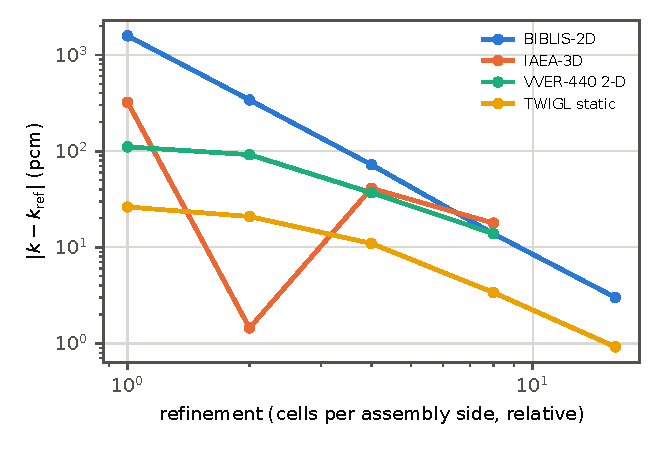
\includegraphics[width=0.62\textwidth]{validation.pdf}
\end{center}
\caption{Eigenvalue error against mesh refinement for the four benchmarks. IAEA-3D
and TWIGL change sign after the coarsest mesh; the dips mark the crossing, not
higher accuracy.}
\label{fig:validation}
\end{figure}

\begin{itemize}
\item \textbf{BIBLIS} converges from above at about second order, from
  1586~pcm at one cell per assembly to \biblisFine~pcm at sixteen.
\item \textbf{TWIGL} crosses its reference after the coarsest mesh and then
  converges at about second order, to \twiglFine~pcm at 0.5~cm cells.
\item \textbf{IAEA-3D} also crosses: it is 1.4~pcm from the reference at two cells
  per node by cancellation, then $-41$ and $-18$~pcm at four and eight. The GH200
  runs of the FEMFFUSION comparison~\cite{garnetfemffusion} reproduce these
  values to the printed digits and continue to $-5.1$~pcm at 16 and $-1.7$~pcm at
  28 cells per node, with an observed order of 1.96 between 24 and 28.
\item \textbf{VVER-440} converges more slowly, with order 1.4 between the two finest
  meshes, to \vverFine~pcm. Its reference is a FEMFFUSION diffusion solution whose
  own discretization error is not stated, so the remaining difference cannot be
  apportioned between the two codes.
\end{itemize}

A single coarse result is a poor accuracy indicator when the error changes sign;
the convergence sequence is the evidence. One cell per assembly or node is 100 to
1600~pcm off; production calculations need four or more cells per assembly side.

Table~\ref{tab:twigl} compares the TWIGL step (a 2.33\,\% thermal-absorption
reduction in one seed region at $t=0$) and ramp (11.67\,\% over 0.2~s) with the
published powers, which are given to three digits. BDF2 with the steps shown
reproduces them to that precision.

\begin{table}[htbp]
\tablefile{twigl}
\caption{TWIGL transient power relative to $t = 0$, BDF2.}
\label{tab:twigl}
\end{table}

% ---------------------------------------------------------------------------
\section{Application: the HP-MR microreactor}
\label{sec:hpmr}

The HP-MR is the 2~MW$_\mathrm{th}$ heat-pipe microreactor reference design of the
NEAMS Virtual Test Bed~\cite{stauff2024}. Its core holds 30 hexagonal TRISO fuel
assemblies around a central shutdown cell on a 26.752~cm lattice, surrounded by 12
beryllium reflector hexes and 12 rotating control drums: beryllium cylinders
(radius 13.25~cm) carrying a 1~cm B$_4$C layer over a 90$^\circ$ arc. Turning the
arcs towards the core inserts negative reactivity.

\garnet{} rasterizes the core onto the triangular lattice with $6r^2$
triangles per hexagon at refinement $r$, so assembly boundaries are exact
(Figure~\ref{fig:hpmr-geometry}, $r = 6$, \hpmrCellsSix{} triangles). The thin
absorber arc is not resolved by the mesh. Instead, the exact area of the annular
sector inside each triangle is computed in polar coordinates and the B$_4$C is
volume-mixed into the cell, so the absorber area is exact at any refinement and
varies continuously with the drum angle.

\begin{figure}[htbp]
\begin{center}
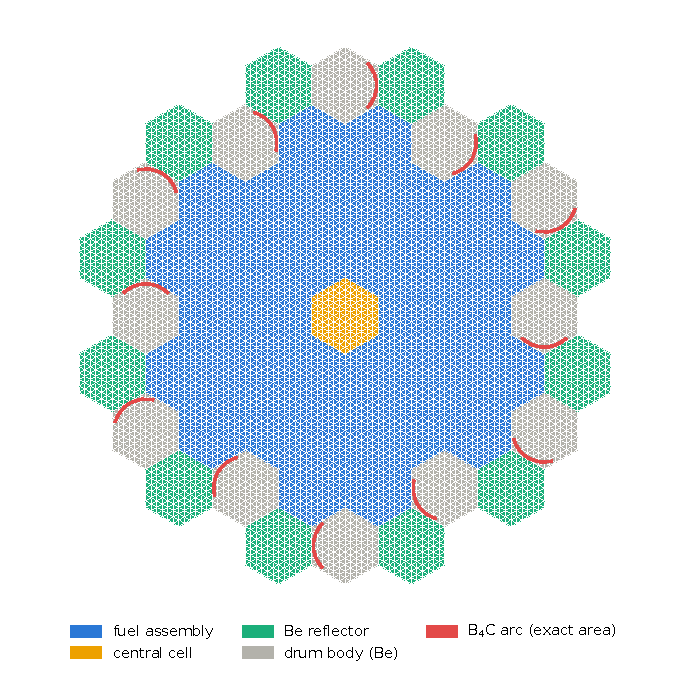
\includegraphics[width=0.55\textwidth]{hpmr_geometry.pdf}
\end{center}
\caption{The 2-D HP-MR model at refinement 6, drums at 90$^\circ$. Every triangle is
one finite-volume cell; the red arcs are the exact absorber areas mixed into the
drum cells. Outside the drum ring is vacuum.}
\label{fig:hpmr-geometry}
\end{figure}

The calculations below use the 11-group ENDF/B-VIII.0 constants shipped with
\garnet{}, with the fuel assemblies homogenized by flat-flux volume weighting.
They are diffusion results without equivalence (SPH) correction, so they show
the numerical behaviour of the model, not the reactor's drum worth. Table~\ref{tab:hpmr} and
Figure~\ref{fig:hpmr-worth} give $k$ and the reactivity relative to the withdrawn
state (180$^\circ$) at three refinements.

\begin{table}[htbp]
\tablefile{hpmr}
\caption{2-D HP-MR, 11 groups: $k$ and reactivity $\rho = 10^5(1/k_{180} - 1/k)$
against drum angle at refinements $r$.}
\label{tab:hpmr}
\end{table}

\begin{figure}[htbp]
\begin{center}
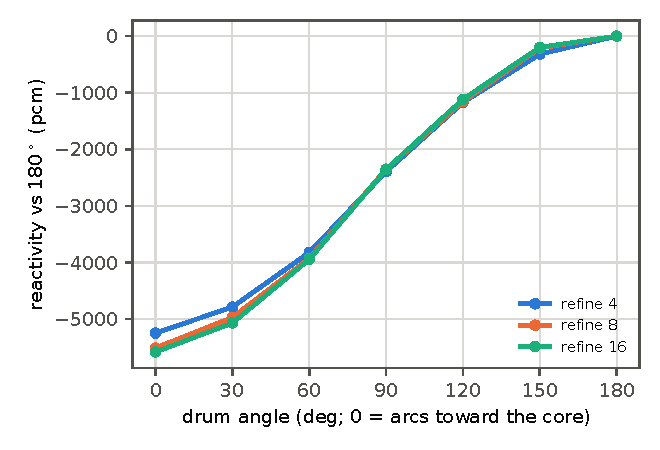
\includegraphics[width=0.62\textwidth]{hpmr_worth.pdf}
\end{center}
\caption{Drum-worth curve, all twelve drums rotated together.}
\label{fig:hpmr-worth}
\end{figure}

The curve has the expected S-shape: flat while the arcs face outward, steepest
at mid rotation. Its magnitude, however, is not mesh-converged.
Table~\ref{tab:hpmr-series} extends the end angles to refinement 32 (0.48~cm
triangles, run on an A100) and adds a control with the B$_4$C replaced by drum
beryllium.

\begin{table}[htbp]
\tablefile{hpmr_series}
\caption{HP-MR mesh series: $k$ at the end angles, total worth
$10^5(1/k_0 - 1/k_{180})$ and its change per refinement, and $k$ at 0$^\circ$ with
the absorber removed. ``Side'' is the triangle edge.}
\label{tab:hpmr-series}
\end{table}

\begin{itemize}
\item \textbf{Without the absorber the model is converged.} $k$ varies by
  \noabsSpread~pcm from refinement 4 to 32: the fuel, reflector and drum bodies
  are resolved on the coarsest mesh.
\item \textbf{With it, the worth is not.} The total worth moves from
  \hpmrWorthCoarse{} to \hpmrWorthFine~pcm and still changes by about 170~pcm
  between refinements 16 and 32.
\item \textbf{Why.} The B$_4$C layer is 1~cm thick, but in the six thermal groups its
  diffusion length $\sqrt{D/\Sigma_r}$ is 0.002 to 0.05~cm, ten to two hundred times
  smaller than the finest triangles. The flux gradient inside the absorber is not
  resolved, and diffusion theory itself is not valid over such distances.
\end{itemize}

Explicit absorber arcs in a diffusion model therefore do not give a drum worth by
mesh refinement. Table~\ref{tab:hpmr-cost}
gives the cost per solve. These solves take 220--340 outer iterations with the
default Anderson-accelerated power iteration; the Wielandt shift was not used.

\begin{table}[htbp]
\tablefile{hpmr_cost}
\caption{Cost per HP-MR eigenvalue solve: mean over the seven angles on one CPU
core (refinements 4--16) and over the two end angles on one A100 (refinement 32),
one run each.}
\label{tab:hpmr-cost}
\end{table}

\subsection{Drum worth through SPH-DF equivalence}

The production route keeps diffusion everywhere but takes its constants from
triangular S$_N$ references with P$_2$ scattering. Flux--volume SPH factors with
discontinuity factors on the vacuum faces (SPH-DF) are computed on equivalence
zones built for drum cores: each drum split into a core and eight ring sectors
aligned on its outward line, beryllium-only outer layers, and boundary hexes
split into inner and outer parts, with no B$_4$C in a boundary zone. The
results below are those of the SPH audit~\cite{sphaudit} (Sections 10.6--10.9),
quoted here, not recomputed:
\begin{itemize}
\item \textbf{Statics.} At every table angle SPH-DF reproduces the reference $k$ and
  every zone rate with drum factors between 0.3 and 3.6. Tables every 5$^\circ$,
  interpolated linearly in angle and evaluated at 20 off-table angles against
  refinement-32 S$_N$ references, give a worst $|\Delta k|$ of 35~pcm, a worst
  assembly power error of 0.30\,\%, a pin RMS of 0.27\,\% and a worst pin of
  2.3\,\%.
\item \textbf{Transients.} With 2.5$^\circ$ tables the SPH-DF model reproduces full
  space--time S$_N$ transients of all twelve drums (a +\$0.27 ramp in 0.2~s, and a
  withdrawal-to-insertion rotation reaching $-$\$5.9 at 1~s) to 0.25\,\% in final
  power and 0.4\,\% in energy. The remaining peak errors of 1.2--3.2\,\% follow the
  reference mesh's own ripple of $k$ in angle.
\end{itemize}
The modelling defaults for drum cores (zoning, tables, local refinement of the
drum band) are recorded with the audit.

% ---------------------------------------------------------------------------
\section{Limits of this report and further reading}
\label{sec:further}

\begin{itemize}
\item \textbf{Diffusion near strong absorbers.} Explicit thin absorbers do not
  converge with the mesh (Section~\ref{sec:hpmr}); drum cores use S$_N$ references
  and SPH-DF equivalence, documented in the SPH audit. Small, leaky cores call for
  SP$_N$ or S$_N$.
\item \textbf{Transient coverage.} Adaptive time stepping and the higher-order BDF
  schemes are available for diffusion; SP$_N$ transients are backward Euler only.
\item \textbf{One device.} Multi-GPU execution is not part of the code.
\end{itemize}

Related reports in the repository:
\begin{itemize}
\item SP$_N$/SDP$_N$ against Carre\~no et al.\ (Brantley--Larsen, C5G7):
  \path{benchmark-results/carreno2024-sdpn-vv/carreno2024-sdpn-vv.pdf};
\item \garnet{} against FEMFFUSION, time to accuracy on CPU and GH200 (IAEA-3D,
  Langenbuch, 3-D HP-MR):
  \path{benchmark-results/garnet-vs-femffusion/garnet-vs-femffusion.pdf};
\item LRA-2D with feedback and adaptive BDF:
  \path{benchmark-results/lra2d-adaptive-bdf-report/adaptive-bdf-lra-benchmark.pdf};
\item triangular S$_N$ with anisotropic scattering:
  \path{benchmark-results/sn-anisotropic-vv/sn-anisotropic-vv.pdf};
\item Godiva with GeN-Foam data: \path{benchmark-results/godiva-genfoam/godiva-genfoam.pdf};
\item the full verification and validation record: \path{docs/verification_validation.md}.
\end{itemize}

\paragraph{Reproducing this report.} \code{docs/theory/run\_cases.py} computes every
number and writes \code{docs/theory/data}. \code{sbatch docs/theory/run\_cases.sbatch
STUDY...} runs studies on a merlin7 CPU node (about one hour without the two HP-MR
follow-ups); \code{run\_cases\_gpu.sbatch hpmr32 hpmr\_noabs} runs those on an A100
in eight minutes. \code{make} in \code{docs/theory} rebuilds the tables, figures
and this PDF.

\begin{thebibliography}{99}
\bibitem{brantley2000}
P.~S. Brantley and E.~W. Larsen, ``The simplified P$_3$ approximation,''
\emph{Nucl.\ Sci.\ Eng.} 134 (2000) 1--21.

\bibitem{carreno2024}
A.~Carre\~no et al., ``Development of a diffusive simplified double P$_N$
approximation to the neutron transport equation,'' \emph{Ann.\ Nucl.\ Energy}
207 (2024) 110675.

\bibitem{walker2011}
H.~F. Walker and P.~Ni, ``Anderson acceleration for fixed-point iterations,''
\emph{SIAM J.\ Numer.\ Anal.} 49 (2011) 1715--1735.

\bibitem{cherezov2025}
A.~Cherezov, A.~Vasiliev and H.~Ferroukhi, ``Application of backward differential
formula and Anderson's method for multigroup diffusion transient equation,''
\emph{Ann.\ Nucl.\ Energy} 210 (2025) 110837.

\bibitem{finnemann1977}
H.~Finnemann, \emph{Argonne Code Center: Benchmark Problem Book}, ANL-7416
Suppl.~2, Argonne National Laboratory (1977).
\url{https://doi.org/10.2172/12030251}.

\bibitem{hageman1969}
L.~A. Hageman and J.~B. Yasinsky, ``Comparison of alternating-direction
time-differencing methods with other implicit methods for the solution of the
neutron group-diffusion equations,'' \emph{Nucl.\ Sci.\ Eng.} 38 (1969) 8--32.

\bibitem{femffusion}
A.~Vidal-Ferr\`andiz et al., FEMFFUSION, a finite-element neutron diffusion and
SP$_N$ code, \url{https://github.com/Zonni/FEMFFUSION}.

\bibitem{stauff2024}
N.~E. Stauff et al., ``High-fidelity multiphysics modeling of a heat-pipe
microreactor using BlueCrab,'' \emph{Nucl.\ Sci.\ Eng.} (2024),
\url{https://doi.org/10.1080/00295639.2024.2375175}.

\bibitem{garnetfemffusion}
\garnet{} versus FEMFFUSION: time to accuracy,
\path{benchmark-results/garnet-vs-femffusion/garnet-vs-femffusion.pdf}.

\bibitem{vvrecord}
\garnet{} verification and validation record, \path{docs/verification_validation.md}.

\bibitem{sphaudit}
\garnet{} SPH audit, \path{docs/qa/sph_audit_2026-11-13.md}.
\end{thebibliography}

\end{document}
